\documentclass[aspectratio=1610]{beamer}
\usepackage[utf8]{inputenc}
\usepackage{multicol}
\usepackage[czech]{babel}
\usepackage{amsmath}
\usepackage{csquotes}
\usepackage{bold-extra}
\usepackage{listings}
\usepackage{alltt,xcolor}

\title{Základy CSS}
\date{WBA | 9., 10. hodina}
\author[Cajthaml]{Matěj Cajthaml}

\usetheme{material}

\usePrimaryCustom

\begin{document}

\begin{frame}
\titlepage
\end{frame}

\begin{frame}{Obsah prezentace}
    \begin{cardTiny}
        \begin{minipage}{\textwidth}
            \vspace{1ex}
            \tableofcontents
        \end{minipage}
    \end{cardTiny}
\end{frame}



\section{Co je to CSS}

\begin{frameImg}[width]{img/cssrender.png}
    \vspace*{60mm}
    \begin{cardTiny}
        \vspace*{\fill}
        \begin{center}
            \textbf{CSS}
        \end{center}
    \end{cardTiny}
\end{frameImg}

\begin{frame}{CSS}
    \begin{cardTiny}
        \begin{flushleft}
            = \textbf{Cascading Style Sheets}.

            Definice stylů stránky, které jsou nezávislé na HTML.

            Způsob zobrazení (designu) prvků na stránce.

            \vspace{2ex}
            Barva a velikost písma, zarovnání, rámečky, odsazení...
        \end{flushleft}
    \end{cardTiny}
\end{frame}

\begin{frame}
    \begin{center}
        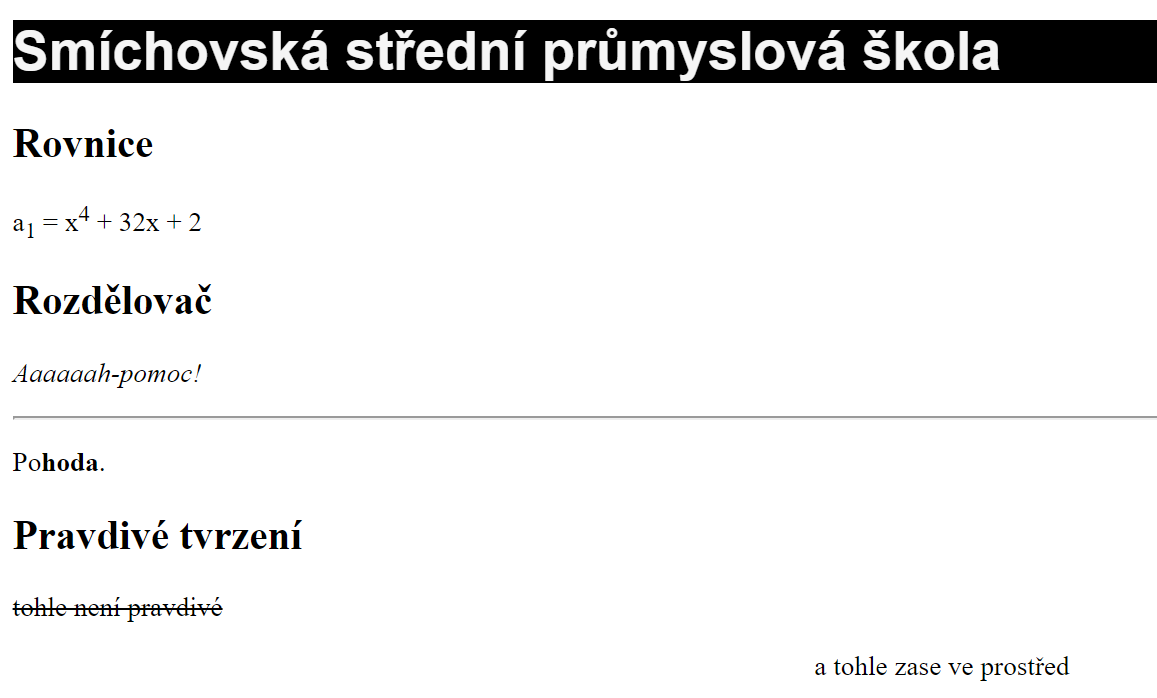
\includegraphics[width=\textwidth]{img/html-7-8-ukol.png}
    \end{center}
\end{frame}

\end{document}